\chapter{Tehnologii utilizate pentru back-end}
\label{sec:proj-backend}
\section{Descrierea arhitecturii}
\label{sec:proj-backend-architecture}

Backend-ul este construit folosind o arhitectură cu microservicii, care permite scalare și
întreținere ușoară. Avem patru servicii principale pentru logică de
produs, un serviciu care funcționează ca router al arhitecturii, două instanțe de baze de date
nerelaționale, un serviciu de gestionare a infrastructurii, un serviciu de monitorizare care
funcționează împreună cu un serviciu de provizionare de metrici și un serviciu de vizualizare de metrici
și în final utilitarele corespunzătoare pentru gestionarea bazelor de date integrate.

S-a ajuns la o asemenea arhitectura pe microservicii deoarece o variantă monolit nu răspundea
bine nevoilor platformei, care are diferite componente cu scop total separat. Ele
comunică foarte puțin între ele, mai mult facând-o cu  frontend-ul printr-un 
router dedicat. În acest mod, s-a putut dezvolta fiecare parte a backend-ului separat, fără
a influența componente deja implementate. Împărțirea pe servicii s-a realizat în funcție de scopul 
principal, făcând diferența între datele utilizatorilor, datele educaționale, codul C++ din fluxul interactiv și altele.

\subsection{Configurarea clusterului}
Clusterul este configurat folosind Kubernetes\footnote{https://kubernetes.io/}, care permite orchestrarea containerelor și
gestionarea resurselor print-o soluție larg folosită. Fiecare serviciu este containerizat folosind Docker,
permițându-ne să rulăm aplicațiile într-un mediu izolat și consistent. Apoi containerele sunt încărcate în Docker,
de unde se poate face lansarea sau oprilea lor în unități logice numite pod-uri. Kubernetes gestionează
scalarea automată a serviciilor, distribuția sarcinilor și asigură disponibilitatea acestora.

Alegerea Kubernetes este justificată de specificul platformei dezvoltate, dar și de publicații precum \cite{k8sBenefits}, care scoate în
evidența avantajele principale ca scalabilitatea crescută, portabilitatea și flexibilitatea pe care o poate
aduce în dezvoltarea și implementarea de platforme Web. Pentru dezvoltare rapidă și locală
s-a folosit Kubernetes în Docker (kind) care a permis îmbinarea și a avantajelor oferite de Docker, putând lansa 
container Docker în Kubernetes după cum am menționat. Acest lucru a ajutat și testarea
codului înainte de a-l lansa în diferite medii.

Dezvoltarea astfel a permis integrarea rapidă a noilor funcționalități și
testarea acestora într-un mediu controlat. De asemenea, a permis simularea unor scenarii de
scalabilitate și performanță, asigurând că platforma poate gestiona un număr mare de
utilizatori și cereri simultane.

Procesul de implementare și lansare presupune construirea imaginilor Docker\footnote{Tehnologie de containerizare
a aplicațiilor software https://www.docker.com/} pentru fiecare
serviciu, încărcarea acestora în registrul de imagini gestionat prin Docker Desktop pentru
testare și apoi reîncărcărea acestora în clusterul Kubernetes. Acest proces este automatizat
prin intermediul unui pipeline CI/CD în mediul de dezvoltare Github. Pentru asta se folosește
GitHub Actions\footnote{https://github.com/features/actions}, care permit rularea automată a diferitelor procese de construire, formatare
și apoi trecerea prin zona de testare și lansare a aplicației.
Practic folosind GitHub Actions, am putut să creăm un flux de integrare și livrare
continuă\footnote{https://www.redhat.com/en/topics/devops/what-is-ci-cd} care a permis să automatizăm
procesul de construire, testare și implementare a platformei.

Fiecare serviciu are propriile fișiere \textit{.yaml}\footnote{Fișiere de configurare, în limbaj de marcaj}
care definesc după caz modul de rulare, variabilele de mediu,
resursele necesare, rutarea, porturile expuse și alte setări specifice.


\subsection{Structurarea şi crearea fişierelor YAML}

Pentru fiecare componentă a backend‐ului (\texttt{Deployment}, \texttt{Service}, 
\texttt{Ingress}, \texttt{ConfigMap}, \texttt{PersistentVolumeClaim}) s-au creat fişiere YAML
separate în directoarele \file{./k8s/} ale fiecărui serviciu. Denumirea fișierelor corespunde resursei Kubernetes pe care o gestionează.

S-au folosit
*-deployment.yaml\footnote{https://kubernetes.io/docs/concepts/workloads/controllers/deployment/},
*-service.yaml\footnote{https://kubernetes.io/docs/concepts/services-networking/service/},
*-ingress.yaml\footnote{https://kubernetes.io/docs/concepts/services-networking/ingress/},
*-configmap.yaml\footnote{https://kubernetes.io/docs/concepts/configuration/configmap/} și
*-pvc.yaml\footnote{https://kubernetes.io/docs/concepts/storage/persistent-volumes/}.

Fișierele de Deployment pentru servicii sunt structurate astfel încât să definească
propietățile principale ale serviciului, cum ar fi numele, etichetele,
numărul de replici, selectorul de etichete și specificațiile containerelor.
\begin{lstlisting}[style=yamlstyle]
apiVersion: apps/v1, kind: Deployment
metadata: name, labels
spec: replicas: 1, selector: matchLabels: app, template:
  metadata: labels: app, spec: name, image: .., ports, env: ..
\end{lstlisting}

Acesta este un exemplu de specificații din Deployment-ul pentru unul dintre servicii, cu o singură replică pentru rulare.
El specifică imaginea Docker care va fi utilizată. De asemenea, definește variabilele de mediu necesare (ca cele de conectare
la baza de date MongoDB).

\subsubsection*{Tipuri de resurse şi rolurile lor}

\textbf{Service} (\texttt{kind:Service}): expune pod-urile pe un IP intern al clusterului.
Astfel, alte servicii pot comunica cu acesta prin numele său și portul specificat. Accesul
din exterior nu este permis direct. Astfel se ralizează o comunicare internă sigură între 
servicii, iar accesul exterior e permis prin intrarea unică în Kong Gateway. Putem observa
structura fișierului de configurație pentru un acest tip de serviciu.
\begin{lstlisting}[style=yamlstyle]
apiVersion: v1, kind: Service
metadata: name
spec: type, selector: app, ports: port: 8080, targetPort: 8080
\end{lstlisting}

\textbf{Ingress} (\texttt{kind:Ingress}): defineşte rutarea HTTP/S prin controller-ul folosit.
Acesta permite expunerea serviciilor către exterior printr-un singur punct de intrare și permite
gestionarea traficului prin reguli de rutare, posibile firewalls sau balansarea încărcării pe 
servicii. Acest Ingress poate fi adăugat apoi în configurarea 
oricărui alt serviciu. S-au testat ambele variante cu trunchere a căii sau fără,
dar s-a ales cea fără trunchere a căii pentru a permite accesul direct la un serviciu
anume printr-un cuvânt cheie în URL. Și varianta cu trunchere ar fi funcționat, dar
ar fi existat un număr foarte mare de rute în radăcina ruterului Kong, ceea ce ar fi
putut duce la probleme de gestionare sau posibile conflicte de nume.
\begin{lstlisting}[style=yamlstyle]
apiVersion: networking.k8s.io/v1, kind: Ingress
metadata: name, annotations: konghq.com/strip-path: "false"
spec: ingressClassName, rules: - http: paths: - path, backend: service: name, port
\end{lstlisting}

\textbf{ConfigMap\footnote{https://kubernetes.io/docs/concepts/configuration/configmap/} \& 
PVC\footnote{https://kubernetes.io/docs/concepts/storage/persistent-volumes/}}:
ConfigMap este folosit pentru configurări directe (de ex. pentru serviciul de provizionare
\texttt{prometheus.yml}) şi PVC este folosit de exemplu pentru volumul serviciului de vizualizare a metricilor în
Grafana. Putem observa structura de configurare a celor două tipuri adiționale de resurse.
  \begin{lstlisting}[style=yamlstyle]
apiVersion: v1, kind: ConfigMap
metadata: name, data: prometheus: global: scrape_int, eval_int
---
apiVersion: v1, kind: PersistentVolumeClaim
metadata: name, spec: accessModes, res: requests: storage
\end{lstlisting}

Fiecărei resurse îi corespunde un singur fişier YAML care conţine versiunea api-ului, tipul resursei kind,
metadatele şi specificațiile. Acestea pot fi aplicate cu \cmd{kubectl apply -f <fișier>}, sau
automatizat printr-un pipeline de integrare continuă / livrare continuă (CI/CD) cum am discutat anterior.

\subsection{Gestionarea clusterului}

Clusterul este creat și gestionat după cum s-a prezentat în primul rând cu Kubernetes, folosind manifesturi YAML.
Pe lângă linia de comandă, am integrat Portainer\footnote{https://www.portainer.io/},
pentru o interfață web de administrare. Portainer rulează ca un Deployment sub
serviciul portainer-sa, căruia i s-a atribuit un ClusterRole\footnote{https://kubernetes.io/docs/reference/access-authn-authz/rbac/}
cu toate privilegiile şi un ClusterRoleBinding aferent. Manifestele corespunzătoare (portainer-sa,
portainer-role, portainer-deployment, portainer-rolebinding,
service şi portainer-ingress) sunt folosite pentru configurare și
gestionare a accesului Portainer în cluster. Interfața Portainer, expusă printr-un Service
şi un Ingress pe ruta /portainer, permite vizualizarea nodurilor, pod-urilor, volumelor şi
gestionarea configurațiilor (scalare, relivrare, mesaje) fără comenzi complexe, oferind
în acelaşi timp controale RBAC\footnote{Controlul accesului bazat pe roluri} şi monitorizare centralizată.

Se poate vedea în imaginea de mai jos cum arată interfața Portainer pe clusterul platformei:
\fig[width=1\textwidth]{imgs/portainerlanding.png}{fig:portainer-landing}{Interfața Portainer pe cluster}

Și mai jos se poate observa lista de servicii in linie de comandă versus în Portainer:

\begin{figure}[htb]
  \centering
  \subfloat[Serviciile în Portainer\label{fig:portainer-fullscreen}]{
    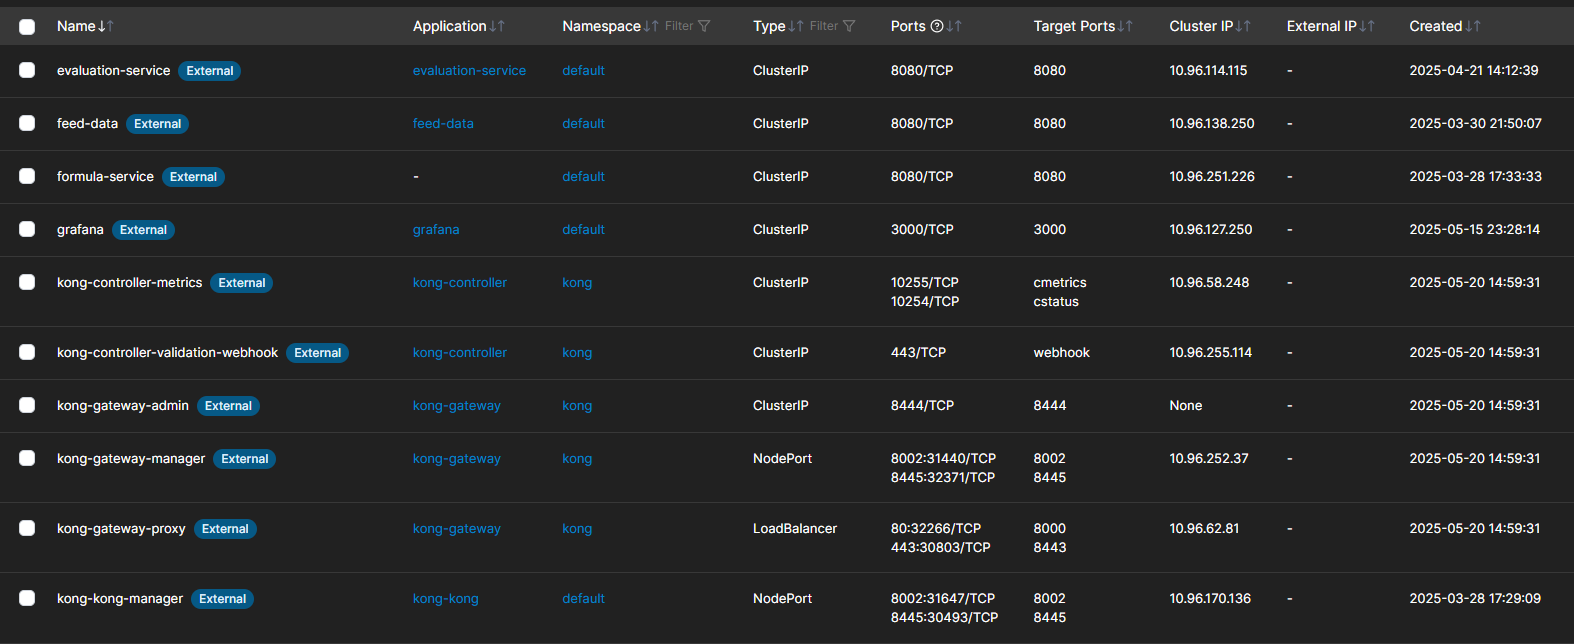
\includegraphics[width=0.48\textwidth]{imgs/servicesportainer.png}
  }
  \hfill
  \subfloat[Serviciile în linie de comandă\label{fig:portainer-cli}]{
    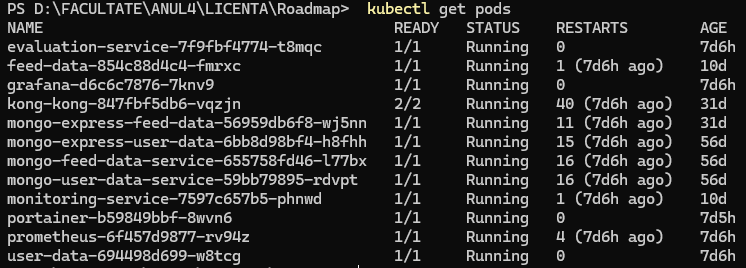
\includegraphics[width=0.48\textwidth]{imgs/servicescli.png}
  }
  \label{fig:portainer-sidebyside}
\end{figure}

\subsection{Rutarea și gestionarea traficului}

Pentru a centraliza şi controla traficul HTTP/S, am ales Kong\footnote{https://konghq.com/} ca API Gateway. În cluster s-a
definit o clasă de rutare dedicată după configurarea Kong ca serviciu separat și s-a adăugat această
clasă în manifestele fiecărui serviciu ce are nevoie de expunere.

Controller-ul Kong va intercepta toate resursele de tip \texttt{Ingress} care 
specifică numele clasei kong. În mediul de dezvoltare, pentru a nu expune un 
LoadBalancer\footnote{https://kubernetes.io/docs/concepts/services-networking/}
extern, am folosit 
port-forwarding\footnote{https://kubernetes.io/docs/tasks/access-application-cluster/port-forward-access-application-cluster/}
local prin:

\noindent
\cmd{kubectl port-forward svc/kong-kong-proxy 8000:80}

Astfel, apelurile HTTP către portul 8000 local sunt tunelate prin Kong şi pot 
fi testate rapid în legătură cu serviciile din cluster fără configurări suplimentare de reţea.

\section{Descrierea serviciilor}


În continuare sunt listate serviciile care alcătuiesc backend-ul aplicației, fiecare având responsabilități specifice
în cadrul arhitecturii pe microservicii.

  \texttt{evaluation-service} – Serviciul pentru gestionarea logicii de creare, monitorizare, deschide/închidere,
  ștergere, gestionare de teste și evaluări. Funcționează ca un controller REST API care preia datele din bazele de date,
  le modelează pentru a fi transmise către frontend și încapsulează și logica de calculare și trimitere către stocarea
  persistentă de punctaje, scoruri, clasamente și alte statistici.

   \texttt{feed-data} – Serviciul care se ocupă de gestionarea datelor legate de secțiunile educaționale și 
  accesarea motorului de generare a moleculelor de chimie. Datele brute din fișierele .mol\footnote{Fișiere de descriere a
  moleculelor chimice} ajung în acest serviciu și sunt parsate linie cu linie pentru a identifica poziția atomilor,
  legăturile chimice dintre ele, tipul lor, dimensiunile și tipul moleculelor. Datele sunt apoi
  transmise către routerul serviciului pentru a fi accesibile prin API-ul REST către frontend.

   \texttt{cpp-compiler-service} – Serviciul care încapsulează logica de gestionare a compilării codului C++
  inserat în editorul interactiv și îl împarte în capturi de status a structurilor de date ce apar. Codul
  este primit din frontend și trece prin mai multe etape de procesare. Se trece linie cu linie prin el pentru a identifica
  structurile de date folosite și a le extrage. Al doilea pas este de creare și adăugare a unui antet de urmărire a
  fiecărei structuri de date capabil să înregistreze și raporteze statusul la fiecare operație. La ultimul pas 
  aceste statusuri sunt adnotate cu metadatele necesare și inserate cronologic într-o listă de evenimente ca să
  fie trimisă apoi către frontend.

  \texttt{grafana} – Utilitar pentru vizualizarea metricilor și a datelor de monitorizare. Practic este gazdă pentru
  rularea imaginii de Grafana\footnote{https://grafana.com/} care primește metricile colectate de Prometheus\footnote{https://prometheus.io/} 
  și le afișează într-o interfață web.

  \texttt{kong-kong} – Serviciul găzdă pentru controller-ul Kong de gestionarea a rutării și a API-urilor despre care s-a discutat anterior.
  

  \texttt{mongo-express-feed-data} – Interfață web pentru gestionarea bazei de date a feed-urilor educaționale. Oferă
  o interfață grafică pentru vizualizarea și manipularea datelor din baza de date MongoDB asociată cu serviciul de feed-uri.
   
  \texttt{mongo-express-user-data} – Interfață web pentru gestionarea bazei de date a utilizatorilor. Oferă ca și cea
  anterior menționată o interfață grafică pentru vizualizarea și manipularea datelor din baza de date MongoDB asociată
  cu serviciul de utilizatori.

   \texttt{mongo-feed-data-service} – Baza de date MongoDB pentru serviciul de feed-uri educaționale.
   
   \texttt{mongo-user-data-service} – Baza de date MongoDB pentru serviciul de utilizatori.
   
   \texttt{monitoring-service} – Serviciul de monitorizare care colectează și expune metrici. Practic aici se încapsulează
  parțile de cod care folosesc instrumentarea oferită de Prometheus pentru a crea interfețe reutilizabile ce vor fi inserate
  în zonele din celelalte servicii unde se dorește colectarea de metrici.
   
  \texttt{portainer} – Interfață de administrare a clusterului Kubernetes. Oferă toate operațiile posibile pentru
  operarea cu resursele din cluster.
   
  \texttt{prometheus} – Serviciul care este gazdă pentru imaginea de Prometheus\footnote{https://prometheus.io/} 
  folosită în seriviciul de monitorizare.
  
  \texttt{user-data} – Serviciul pentru gestionarea datelor utilizatorilor, 
  inclusiv autentificare și autorizare. El funcționeză ca un router REST API care are mai multe straturi prin care trec datele.
  Primul este cel de validare a token-ului de autentificare în middleware-ul JWTAuth, apoi prin parsarea datelor,
  stocarea lor persistentă în baza de date MongoDB și apoi prin reexpunerea lor către frontend prin API-ul REST.

Mai jos în figura \ref{fig:arhitectura-backend}
putem observa și arhitectura principală de comunicare între serviciile din back-end.
\fig[width=0.85\textwidth]{imgs/bediagram.png}{fig:arhitectura-backend}{Arhitectura backend-ului aplicației}


\subsection{Descrierea API-urilor}

Fiecare serviciu are un API RESTful care permite interacțiunea cu resursele sale.
Aceste API-uri sunt definite în routerul fiecărui serviciu care este creat prin biblioteca Gorrilla Mux în Go.
Fiecare serviciu are un set de endpoint-uri care permit operații CRUD (Create, Read, Update, Delete) asupra resurselor sale
și interacționează cu baza de date corespunzătoare.

\section{Securitate}

Toate API-urile serviciilor sunt protejate prin JWT\footnote{JSON Web Token, folosit în protocoale de autentificare}, validat de
secțiunea JWTAuth, care
respinge cererile fără token sau cu token invalid. Traficul extern este dirijat prin Kong după cum am văzut,
configurat cu HTTPS/TLS, politici de limitare a numărului de cereri HTTP, CORS\footnote{Cross-Origin Resource Sharing}
şi trunchere a căii pentru a preveni
atacurile de tip „path traversal”\footnote{Atacuri bazate pe manipularea căii de acces a resurselor} şi abuzul de resurse.
În interiorul clusterului, rolurile
şi permisiunile sunt gestionate prin RBAC Kubernetes (ClusterRole/ClusterRoleBinding\footnote{https://kubernetes.io/docs/reference/access-authn-authz/rbac/}), iar
Portainer rulează sub un ServiceAccount cu drepturile strict necesare la acces. Conexiunile la bazele
MongoDB sunt realizate folosind URL-urile securizate (MONGO_URI) şi logare cu credențiale
la serverul de baze de date.

\section{CI/CD}

\subsection{Port forwarding}

În mediul de dezvoltare, pentru a testa rapid Ingress‐ul Kong fără LoadBalancer extern, se folosește port‐forwarding
după cum am discutat la capitolul Rutarea și gestionarea traficului. Acest lucru permite accesul la serviciile 
din cluster. Ca pipeline-ul din GitHub Actions să aibă acces la clusterul Kind local s-a folosit
un runner GitHub hostat 
local\footnote{https://docs.github.com/en/actions/hosting-your-own-runners/about-self-hosted-runners}.
Acesta permite direct accesul la comenzile de build și push în Docker și mai ales la cele de redeploy
al serviciilor în cluster.

\subsection{Deployment}

După cum am menționat am automatizat build-ul, testarea şi deploy-ul în Kubernetes cu GitHub Actions.
\begin{itemize}
  \item \textbf{Checkout \& Context:} se selectează codul pentru fiecare serviciu şi se setează contextul kubectl 
  la \texttt{kind-visioscience}, clusterul unde rulează local mediul de dezvoltare.
  \item \textbf{Build \& Push Docker:} se compilează binarele Go, se construiește imaginea cu build-push-action
  şi se încarcă pe DockerHub sub numele <user>/\texttt{\$SVC:latest}.
  \item \textbf{Deploy:} rulăm:
    \begin{lstlisting}[style=yamlstyle]
kubectl apply -f k8s/
kubectl rollout status deployment/extract.outputs.name
    \end{lstlisting}
  \item Runner-ul GitHub este un hostat pe aceeaşi mașină ca și clusterul Kind, astfel că are acces direct la 
kubeconfig\footnote{https://kubernetes.io/docs/concepts/configuration/organize-cluster-access-kubeconfig/}.
\end{itemize}

\subsection{Metrici / Monitorizare}

\subsection{Avantajele folosirii Prometheus}

Prometheus este un sistem de monitorizare și alertare foarte popular în mediile moderne de dezvoltare și producție
datorită scalabilității și flexibilității sale. Oferă o arhitectură simplă bazată pe
colectarea activă a metricilor prin intermediul unor endpoint-uri HTTP expuse de aplicații,
facilitând integrarea rapidă cu o varietate largă de
servicii și microservicii. În plus, arhitectura sa detașată de stare (stateless) și suportul
pentru stocarea pe termen scurt cu export către sisteme
externe îl fac ideal pentru arhitecturi dinamice, precum în Kubernetes. De asemenea, se integrează
nativ cu instrumente vizuale precum Grafana, oferind dashboard-uri ușor de configurat
și interpretat de către dezvoltatori. Grafana e o soluție ideală pentru vizualizarea metricilor
colectate de Prometheus, fapt menționat și în publicații precum \cite{grafanaObs}, care îl descrie 
ca o necesitate esențială în platformele moderne.

\subsection{Colectare Prometheus}  
În fiecare serviciu Go am folosit clientul official Prometheus:

\texttt{github.com/prometheus/client\_golang/prometheus} pentru definirea contoarelor, 
histogramelor şi gauge-urilor.

\texttt{github.com/prometheus/client\_golang/prometheus/promhttp} pentru expunerea 
endpoint-ului \texttt{/\$SERVICIU/metrics}.

De exemplu, în \texttt{evaluation-service} în codul responsabil de metrici definim astfel. 
\begin{lstlisting}[style=yamlstyle]
registry := prometheus.NewRegistry()
reqTotal := prometheus.NewCounterVec(...)
registry.MustRegister(reqTotal, reqDuration, activeEvals)
http.Handle("/eval/metrics", HandlerFor(registry, opt))
\end{lstlisting}

\subsection{Grafana Dashboard}  
De exemplu după ce Prometheus trece prin \texttt{evaluation\_service\_http\_requests\_total}, se crează un dashboard 
persistent prin volumele Kubernetes. Dashboard-ul Grafana are în general două tipuri de panouri pentru metrici 
similare. De exemplu pentru metrica de cereri și evaluări active din serviciul de evaluare:

Timeseries (serie temporală de date) pentru \texttt{eval\_svc\_req\_total}.

Gauge (serie de valori) pentru \texttt{eval\_svc\_active\_evals}.

Iar apoi ele sunt definite și legate în configurația panoului din Grafana.
\begin{lstlisting}[style=yamlstyle]
  "panels":
     {"type":"timeseries",
      "targets":[{"expr":"eval_svc_req_total"}],
      "title":"HTTP Total Requests"}, ....
\end{lstlisting}
Aceste panouri sunt importate în Grafana în \texttt{Evaluation Service Dashboard} şi actualizate
la fiecare 5s (configurabil).

Așadar există trei panouri principale în Grafana pentru trei servicii de logică de produs existente:
  
  \texttt{Evaluation Service Dashboard} pentru \texttt{evaluation-service}
  \fig[width=1\textwidth]{imgs/evaluationdashboard.png}{fig:evaluation-dashboard}{Dashboard-ul pentru evaluări în Grafana}
  
  Se poate observa logarea numărului de cereri HTTP din serviciu, latența și durata medie a lor, numărul de evaluări
  active și rata operațiilor pe evaluări.

  \texttt{Feed Data Service Dashboard} pentru \texttt{feed-data}
  
  În panou se pot vedea numărul de cereri HTTP, latența și durata medie a lor, numărul de feed-uri active, numărul de molecule
  active, rata operațiilor asupra feed-urilor și moleculelor, precum și numărul de molecule generate. La fel
  ca la cel de evaluări, metricile se împart în cele două categorii discutate.

  \texttt{User Data Service Dashboard} pentru \texttt{user-data}

  Ca și în celelate panouri, și aici apare numărul, latența și durata cererilor HTTP. Metricile specifice serviciului
  sunt numărul utilizatorilor și al claselor active.
\section{Soluția de baze de date}
\label{sec:proj-database}

\subsection{Structura bazei de date}

\subsubsection{Tipuri de baze de date utilizate / Motivația alegerii}

Baza de date folosită este MongoDB\footnote{https://www.mongodb.com/}, o bază de date nerelațională care oferă flexibilitate și scalabilitate
și e ușor de folosit și mai ales de integrat în microserviciile gestionate în Kubernetes. Am ales o soluție
nerelațională deoarece datele noastre sunt semi-structurate și nu necesită relații complexe între tabele,
permițându-ne să stocăm documente JSON care pot fi ușor extinse și modificate fără a necesita migrări
de baze de date. Structura se putea să fie integrată și într-un mediu relațional, dar am considerat că
MongoDB oferă o flexibilitate mai mare pentru tipurile de date pe care le gestionăm, cum ar fi feed-urile 
educaționale, datele utilizatorilor, cât și pentru structura testelor și evaluărilor.

Avantajele folosire MongoDB sunt descrise și în publicații precum \cite{mongoDevTo}, care menționează
flexibilitatea schemelor și pe de altă parte scalabilitatea și performanța pe care o oferă ca avantaje majore. 
Având în vedere nevoile platformei dar și avantajele menționate și aici și în articolul dat,
MongoDB este justificat o alegere bună în cazul proiectului de față.

Un alt avantaj al folosirii MongoDB este că permite stocarea datelor într-o formă 
orientată pe documente similare cu JSON. Alegerea s-a bazat și pe flexibilitatea schemelor,
scalabilitatea orizontală și compatibilitatea nativă cu structurile de date folosite, precum și
pe posibilitatea de a face agregări complexe și de a gestiona relații parțiale între documente. 

\subsubsection{Gestionarea datelor}

Datele sunt organizate în colecții care corespund entităților sistemului:
quiz-uri, formule, molecule, utilizatori, clase, invitații, etc. Fiecare colecție conține documente ce
respectă structurile definite în codul backend-ului, folosind driverul oficial MongoDB pentru
Go (go.mongodb.org/mongo-driver).

De exemplu, un document din colecția quizzes conține câmpuri precum Title,
ClassID și OwnerID (reprezentate prin id de obiect din MongoDB), un array de
Questions cu întrebări, răspunsuri și punctaje, și un array QuizResults pentru
stocarea scorurilor utilizatorilor.

Tabelele sunt separate încât să aibă minimă interacțiune între ele, relaționând maxim prin câteva
câmpuri, de obicei id-urile obiectelor din altă colecție. De exemplu, colecția quizzes are
câmpul ClassID care face referire la colecția classes, iar colecția
users are câmpul ClassID pentru a lega utilizatorii de clasele lor. Arhitectura principală a tabelelor din
cele două baze de date folosite se poate observa în figura următoare.

\fig[width=1\textwidth]{imgs/dbdiagram.png}{fig:mongodb-structure}{Structura principală a tabelelor din MongoDB}

Se folosesc structuri Go care reflectă aceste modele, permițând deserializarea și serializarea 
automată între BSON\footnote{https://www.mongodb.com/resources/basics/json-and-bson} și
JSON. Astfel, interacțiunea 
cu baza de date se face prin operații CRUD folosind
metodele MongoDB standard, iar aplicația transformă și face validarea datelor ușor. O problemă
întâmpinată des a fost de confundare a numelui unui cămp la serializare sau deserializare, 
de obicei între numele lui CamelCase și snake_case, dar s-a rezolvat prin implementarea unui
strat de uniformizare a structurilor.

Gestionarea și vizualizarea datelor în mediul de dezvoltare a fost facută folosind interfețele oferite de Mongo express,
care permit toate operațiile cu documentele din colecțiile MongoDB printr-o interfață web simplă și intuitivă.

\subsection{Securitatea datelor}

Datele stocate sunt protejate prin controlul accesului la nivel de cluster MongoDB, autentificare
și autorizare prin roluri definite (de exemplu, utilizator, profesor).
Parolele sunt criptate și gestionate prin variabile de mediu la nivelul serviciilor. Pe viitor 
se poate face integrarea cu un serviciu de autentificare centralizat (ex: OAuth2, OpenID Connect)
sau folosirea unui serviciu de identitate și secrete (precum HashiCorp Vault sau AWS Secrets Manager) pentru a gestiona
securitatea și accesul și mai granular la datele sensibile.

\subsubsection{Performanța și scalabilitatea bazei de date}

MongoDB permite scalarea orizontală prin sharding\footnote{https://www.mongodb.com/docs/manual/sharding/}, facilitând distribuția datelor pe mai multe noduri când 
cantitatea datelor ar ajunge la dimensiuni mari. Indecșii sunt definiți pe câmpuri critice 
(ex: \texttt{\_id}, \texttt{class\_id}) pentru a optimiza căutările și interogările.

De asemenea, conexiunile sunt gestionate eficient prin pool-uri în clientul Go, iar operațiile
lungi sunt efectuate cu timeout-uri pentru a evita blocarea serviciilor sau cu reîncercare pentru
resursele vitale.

\subsection{Integrarea cu back-endul}

Back-endul este implementat în Go, folosind pachetul oficial MongoDB driver, care oferă suport
complet pentru operațiile pe colecții și documente, tranzacții și agregări. 

La pornire, fiecare serviciu inițializează o conexiune persistentă la baza de date. Modelele Go
definite permit maparea clară între structurile din cod și documentele mongo.
De exemplu, în \texttt{evaluation-service}, obiectele \texttt{Quiz} și \texttt{QuizResult}
sunt manipulate direct în cod, iar metodele expun un API REST pentru aceste resurse prin CRUD\footnote{Create, Read, Update, and Delete}.


